\documentclass[9pt, t, aspectratio=169]{beamer}

%~~~~~~~~~~~~~~~~~~~~~~~~~~~~~~~~~~~~~~~~~~~~~~~~~~~~~~~~~~~~~~~~~~~~~~~~~~~~~~
\usepackage[sfdefault]{roboto}
\usepackage[utf8]{inputenc}
\usepackage[T1]{fontenc}
%~~~~~~~~~~~~~~~~~~~~~~~~~~~~~~~~~~~~~~~~~~~~~~~~~~~~~~~~~~~~~~~~~~~~~~~~~~~~~~

%~~~~~~~~~~~~~~~~~~~~~~~~~~~~~~~~~~~~~~~~~~~~~~~~~~~~~~~~~~~~~~~~~~~~~~~~~~~~~~
\usepackage{styles/fluxmacros}
\usefolder{styles}
% Styles: asphalt, blue, red, green, gray 
\usetheme[style=gray]{flux}
%~~~~~~~~~~~~~~~~~~~~~~~~~~~~~~~~~~~~~~~~~~~~~~~~~~~~~~~~~~~~~~~~~~~~~~~~~~~~~~

%~~~~~~~~~~~~~~~~~~~~~~~~~~~~~~~~~~~~~~~~~~~~~~~~~~~~~~~~~~~~~~~~~~~~~~~~~~~~~~
% Zusatzpakete
% Havard zitier stil
\usepackage[square,sort,comma,numbers]{natbib}
% zeilenabstand
\usepackage{setspace}
% mehr zitate
\usepackage{csquotes}
% spacing of enum items
\usepackage{enumitem}

\usepackage{makecell}       % better table formatting
\setitemize{label=\usebeamerfont*{itemize item}%
\usebeamercolor[fg]{itemize item}
\usebeamertemplate{itemize item},
itemsep=1.3em}
% Codeanzeige
\usepackage{listings}
\usepackage{svg}
\usepackage{xcolor}
\usepackage{subcaption}


\definecolor{dkgreen}{rgb}{0,0.6,0}
\definecolor{dkyellow}{rgb}{0.6,0.6,0}
\definecolor{dkblue}{rgb}{0,0,0.6}
\definecolor{dkred}{rgb}{0.6,0,0}
\definecolor{gray}{rgb}{0.5,0.5,0.5}
\definecolor{mauve}{rgb}{0.58,0,0.82}



\lstset{frame=none,
  language=Java,
  aboveskip=0mm,
  belowskip=0mm,
  showstringspaces=false,
  columns=flexible,
  basicstyle={\small\ttfamily},
  numbers=none,
  numberstyle=\tiny\color{gray},
  keywordstyle=\color{dkblue},
  commentstyle=\color{dkgreen},
  stringstyle=\color{dkgreen},
  breaklines=true,
  breakatwhitespace=true,
  numberbychapter=false,
  tabsize=3,
  escapechar=\%
}

\usepackage{booktabs}
\usepackage{colortbl}
\usepackage{ragged2e}
\usepackage{schemabloc}
%~~~~~~~~~~~~~~~~~~~~~~~~~~~~~~~~~~~~~~~~~~~~~~~~~~~~~~~~~~~~~~~~~~~~~~~~~~~~~~

%~~~~~~~~~~~~~~~~~~~~~~~~~~~~~~~~~~~~~~~~~~~~~~~~~~~~~~~~~~~~~~~~~~~~~~~~~~~~~~
% Information
\title{Legal Perspectives on Discrimination}
\subtitle{Robin Schmidt \& Floyd Kretschmar}
\institute{
\includegraphics[width=0.45\textwidth]{assets/uni_logo_dark.png}}
\date{\today}
\titlegraphic{assets/uni_logo.png}
%~~~~~~~~~~~~~~~~~~~~~~~~~~~~~~~~~~~~~~~~~~~~~~~~~~~~~~~~~~~~~~~~~~~~~~~~~~~~~~

\begin{document}

\titlepage

% What are the key points of our talk
\section{Machine Learning and fairness: Key questions}
\begin{frame}{Machine Learning and fairness: Key questions}
    Fundamental questions at the core of fairness discussion in Machine Learning:
    
    \begin{itemize}
        \item Why is fairness in Machine Learning an \textbf{immediately pressing issue}?
        \item Is \textbf{Machine Learning inherently susceptible to unfairness} and why?
        \item What is \textbf{the legal definition of fairness} and how does this perspective inform our view of fairness in Machine Learning?
        \item How can we \textbf{formalize fairness in a mathematical way}?
    \end{itemize}
\end{frame}

% Why does the discussion about fairness matter
\section{Real world impact of ML in terms of fairness}
\begin{frame}{Real world impact of ML in terms of fairness \cite{machinebias}}
    Discussions about fairness in ML are not theoretical: \\
    $\rightarrow$ \textbf{Machine Learning is already used every day to make decisions about peoples lives} \\~\\
    
    \textbf{Example:} Risk assessment tools used to predict the likelihood of committing a future crime
    \begin{itemize}
        \item used in multiple states across the USA
        \item have wide ranging impact on judicial process in the united states: \\
        setting bond amounts, pretrial release, sentencing and parole decisions
    \end{itemize}
    
    \begin{block}{Overall goal of these risk assessment tools}
        \enquote{If computers could accurately predict which defendants were likely to commit new crimes, the criminal justice system could be fairer and more selective about who is incarcerated and for how long.}
    \end{block}
\end{frame}

\begin{frame}{Real world impact of ML in terms of fairness \cite{machinebias}}
    \textbf{But:} \enquote{The trick, of course, is to make sure the computer gets it right.} \\~\\
    
    ProPublica obtained and analyzed risk scores of more than 7,000 people:
    
    \begin{itemize}
        \item \enquote{Only 20 percent of the people predicted to commit violent crimes actually went on to do so.}
        \item \enquote{Of those deemed likely to re-offend, \textbf{61 percent were arrested for any subsequent crimes} within two years.}
        \item \enquote{The formula was particularly \textbf{likely to falsely flag black defendants as future criminals}, wrongly labeling them this way at almost twice the rate as white defendants.}
        \item \enquote{\textbf{White defendants were mislabeled as low risk more often} than black defendants.}
    \end{itemize}
\end{frame}

% What are the underlying dynamics of ML that create unfairness
\section{The Machine Learning Framework: Why is it unfair?}
\begin{frame}{The Machine Learning Framework \cite{Berk.2018}}

    \textbf{Assumption:} Observations are sampled from a joint probability distribution $P(Y, L, S)$ with function $f(L, S)$ linking the predictors to the target variable $Y$
    \begin{itemize}
        \item legitimate predictors L 
        \item protected predictors S
    \end{itemize}
         
    \textbf{Idea:} apply fitting procedure $h(L, S)$ to the data $\Rightarrow$ hypothesis $\hat{f}(L, S)$ that is the source of predictions $\hat{Y}$ \\~\\
    
    $\hat{f}(L, S)$ approximates \dots
    \begin{itemize}
        \item \dots the true response surface in a biased manner
        \item \dots an approximation of the true response surface asymptotically unbiased
    \end{itemize}
\end{frame}

\begin{frame}{The Machine Learning Framework: Why is it unfair? \cite{Barocas.2016, barocas-hardt-narayanan}}
    \underline{\textbf{Target Variable or class Labels:}} \\
    \begin{itemize}
        \item Target variable defines what data miners are looking for (outcome of interest)
        \item Class labels divide all possible values of the target variable into mutually exclusive categories
    \end{itemize}

    \begin{block}{\textbf{Unfairness happening through:}}
    \begin{itemize}
        \item Subjective process (\textbf{e.g.} creditworthiness)
        \item Could be unintentionally be parsed in a way which \textbf{systematically disadvantages} protected classes (\textbf{e.g.} hiring decisions based on predicted tenure than worker productivity)
    \end{itemize}
        \end{block}
\end{frame}

\begin{frame}{The Machine Learning Framework: Why is it unfair? \cite{Barocas.2016, barocas-hardt-narayanan}}
    \underline{\textbf{Training Data:}} Basis of used algorithms and outcome of the model \newline 

    \begin{block}{\textbf{Unfairness happening through:}}
    \begin{itemize}
        \item Biased training data leads to discriminatory models
        \item 1. Cases in which prejudice has played some role
        \item 2. Biased sample of the population (under-/overrepresenttation) leads to skewed results\newline
        $\rightarrow$ less \textbf{accurate}, \textbf{precise} and \textbf{complete} records for certain classes
    \end{itemize}
        \end{block}
\end{frame}

\begin{frame}{The Machine Learning Framework: How is it unfair? \cite{Barocas.2016, barocas-hardt-narayanan}}
    \underline{\textbf{Feature Selection:}} Observed and considered attributes \newline 
    
    \begin{block}{\textbf{Unfairness happening through:}}
    \begin{itemize}
        \item Factors that better account for a protected class are not well represented in the set of selected features 
        \item \textbf{e.g.} hiring decisions, enormous weight to reputation of college (equal competent graduates of protected classes at low rates $\Rightarrow$ individuals get discriminated)
    \end{itemize}
        \end{block}
\end{frame}

\begin{frame}{The Machine Learning Framework: Why is it unfair? \cite{Barocas.2016, barocas-hardt-narayanan}}
    \underline{\textbf{Proxies:}} Non sensitive features correlate to class membership
    \begin{itemize}
        \item Do not artificially introduce discriminatory effects into the data mining process
        \item Can still result in systematically less favorable determinations for members of protected classes
    \end{itemize} 

    \begin{block}{\textbf{Unfairness happening through:}}
    \begin{itemize}
        \item  Redundant Encoding
        \item \textbf{E.g.} same criteria \textbf{correctly sorts} individuals according to their \textbf{predicted likelihood of excelling at a job} also sort individuals according to \textbf{class membership}
    \end{itemize}
        \end{block}
\end{frame}

\begin{frame}{The Machine Learning Framework: Why is it unfair? \cite{Barocas.2016, barocas-hardt-narayanan}}
    \underline{\textbf{Masking:}} Decision makers mask their prejudicial views by using the mentioned methods \newline 
    
    \begin{block}{\textbf{Unfairness happening through:}}
    \begin{itemize}
        \item Bias the collection
        \item Preserve the known effects of prejudice in prior decision making
        \item Use prejudicial features and/or proxies
    \end{itemize}
        \end{block}
\end{frame}

{
\setbeamercolor{background canvas}{bg=gray}
\begin{frame}{Mathematical Perspective: How to quantify Fairness? \cite{Berk.2018}}
\vspace{2cm}
\begin{block}{\huge Overall:}
\LARGE 
    Machine Learning is fundamentally about \textbf{learning from patterns in data}. \\
    If the \textbf{underlying data contains discriminatory patterns}, machine learning algorithms will pick up on those as well, if they are not accounted for.
\end{block}
\end{frame}
}

% How does our understanding of unfairness of ML conflict/overlap with the current legal framework
\section{Legal Perspective: How does ML fit into the current legal framework}
\begin{frame}{Legal Perspective: ML and the current legal framework \cite{Barocas.2016}}
US labor law (Title VII civil rights act) differentiates into \textbf{two kinds} of \textbf{discrimination}: \newline

\begin{block}{\textbf{Disparate treatment} \cite{Barocas.2016, isabel01, isabel02}}
\begin{itemize}
    \item  \textbf{Unequal behavior} towards someone because of a \textbf{protected characteristic} (\textbf{e.g.} race or gender)
    \item \underline{\textbf{ML:}} Different outputs for people with the \textbf{same values} for \textbf{non-sensitive features} but \textbf{different values} for \textbf{sensitive features}
\end{itemize}
\end{block}

\begin{block}{\textbf{Disparate impact} \cite{Barocas.2016, isabel01, isabel02}}
\begin{itemize}
    \item An equal \textbf{neutral rule} \textbf{in form}, but has a \textbf{disadvantageous effect} on some people of a protected characteristic
    \item \underline{\textbf{ML:}} Outputs benefit (hurt) people sharing a value of a protected characteristic
\end{itemize}
\end{block}
\end{frame}

\begin{frame}{Legal Perspective: ML and the current legal framework \cite{isabel01}}
\begin{figure}
    \vspace{1cm}
    \centering
    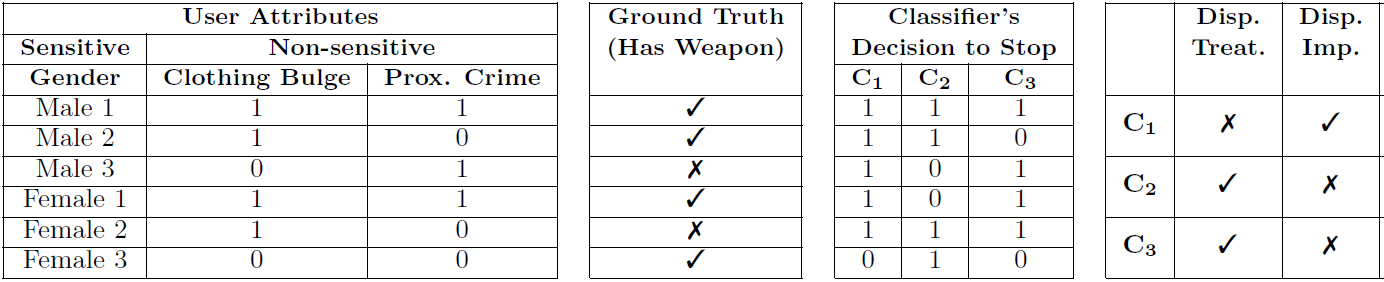
\includegraphics[width=\textwidth]{presentation/assets/DisparateTreatImp.PNG}
    \caption{Decisions of three classifiers whether (1) or not (0) to stop a pedestrian \cite{isabel01, isabel02}}
    \label{fig:exampleDisp}
\end{figure}
\end{frame}

\begin{frame}{Legal Perspective: ML and the current legal framework \cite{isabel01}}
\begin{figure}
    \vspace{1cm}
    \centering
    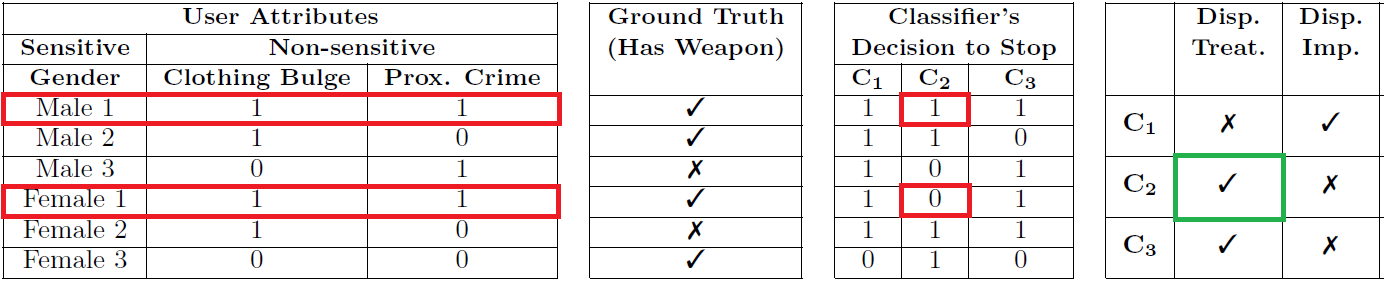
\includegraphics[width=\textwidth]{presentation/assets/DisparateTreatImp(1).png}
    \caption{Decisions of three classifiers whether (1) or not (0) to stop a pedestrian \cite{isabel01, isabel02}}
    \label{fig:exampleDisp1}
\end{figure}
\end{frame}

\begin{frame}{Legal Perspective: ML and the current legal framework \cite{isabel01}}
\begin{figure}
    \vspace{1cm}
    \centering
    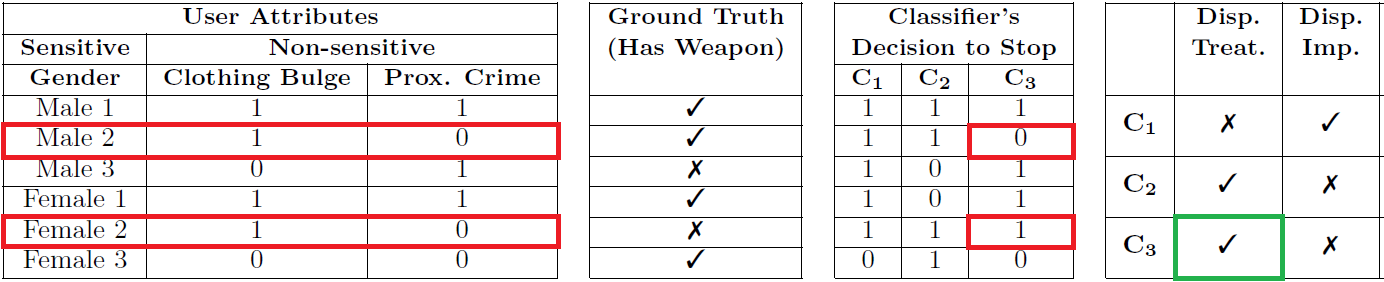
\includegraphics[width=\textwidth]{presentation/assets/DisparateTreatImp(2).png}
    \caption{Decisions of three classifiers whether (1) or not (0) to stop a pedestrian \cite{isabel01, isabel02}}
    \label{fig:exampleDisp2}
\end{figure}
\end{frame}

\begin{frame}{Legal Perspective: ML and the current legal framework \cite{isabel01}}
\begin{figure}
    \vspace{1cm}
    \centering
    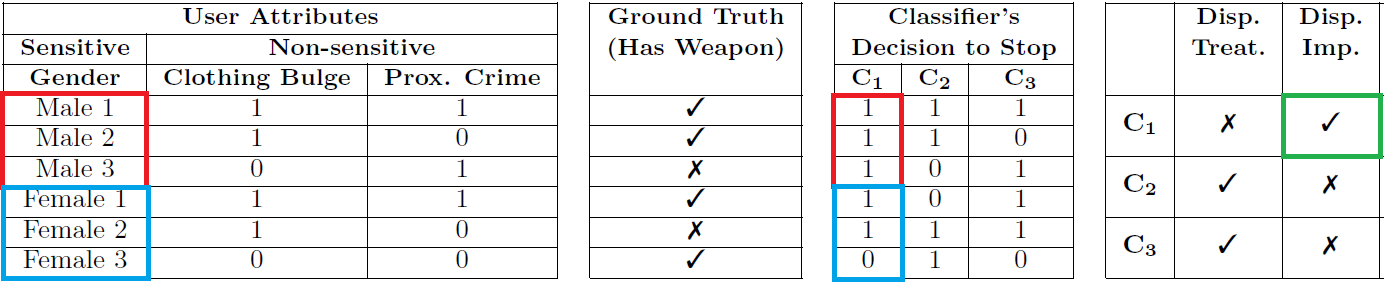
\includegraphics[width=\textwidth]{presentation/assets/DisparateTreatImp(3).png}
    \caption{Decisions of three classifiers whether (1) or not (0) to stop a pedestrian \cite{isabel01, isabel02}}
    \label{fig:exampleDisp3}
\end{figure}
\end{frame}

\begin{frame}{Legal Perspective: ML and the current legal framework \cite{Barocas.2016}}
\underline{\textbf{Liability for disparate treatment:}}\\

\begin{itemize}
    \item Does not correspond to any particular discrimination mechanism within data mining
    \item Classification itself can be legal harm $\Rightarrow$ same should be true for using protected class
    \item Occurs either \textbf{at the decision} to apply a predictive, discriminatory model \textbf{OR} when the \textbf{result is used} for the hiring decision
\end{itemize}
\vspace{1cm}
\underline{\textbf{Overall:}} disparate treatment doctrine does not do much to regulate discriminatory data mining
\end{frame}

\begin{frame}{Legal Perspective: ML and the current legal framework \cite{Barocas.2016}}
\underline{\textbf{Liability for disparate impact:}}\\

\begin{itemize}
    \item Plaintiff must show that a neutral employment practice causes a disparate impact
    \item The defendant-employer may demonstrate that the practice is \textbf{job related} \& a \textbf{business necessity}
    \item Afterwards plaintiff can still show \textbf{alternative employment practice} with \textbf{less discriminatory} results
\end{itemize}
\underline{\textbf{ML:}} Threshold issue is whether or not the target variable is job related\\
\vspace{0.5cm}
$\Rightarrow$ If it's job related: 
\begin{itemize}
    \item[1.] Is the model predictive of that trait?
    \item[2.] Does the model predict what it is supposed to predict? (statistical significance showing that the result of the model correlates to the trait - extremely low bar for data mining)
\end{itemize}
\end{frame}

{
\setbeamercolor{background canvas}{bg=gray}
\begin{frame}{Legal Perspective: ML and the current legal framework \cite{Barocas.2016}}
\vspace{2cm}
\begin{block}{\huge Overall:}
\LARGE Often data mining will both \textbf{predict something meaningful} and have \textbf{disparate impact} (stating a less discriminatory model is often hard)
\end{block}
\end{frame}
}

\begin{frame}{Legal Perspective: ML and the current legal framework \cite{Singh, automatedDsicrimination}}
    \underline{\textbf{Outlook on EU laws:}}\\
    \begin{itemize}
        \item European Convention on Human Rights Article 14 - Prohibits Discriminiation
        \item Charter of Fundamental Rights of the EU Article 21 - Prohibits Discriminiation
        \item Equality law $\Rightarrow$ National Law
    \end{itemize}
    \vspace{0.5cm}
    \underline{\textbf{Some of Protected Characteristics (UK):}}\\[0.75cm]
    \begin{figure}
        \centering
        \begin{subfigure}{.165\textwidth}
            \centering
            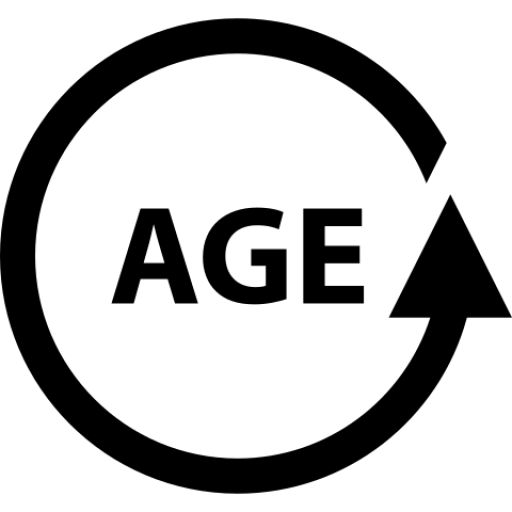
\includegraphics[width=.4\linewidth]{presentation/assets/age.png}
            \caption{AGE}
            \label{fig:sub1}
        \end{subfigure}%
        \begin{subfigure}{.165\textwidth}
            \centering
            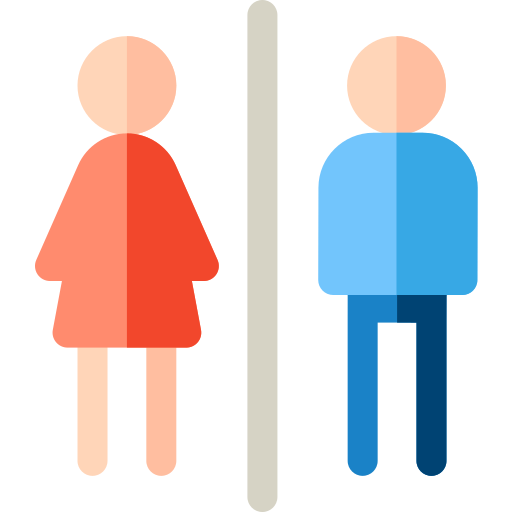
\includegraphics[width=.4\linewidth]{presentation/assets/gender.png}
            \caption{SEX}
            \label{fig:sub2}
        \end{subfigure}%
        \begin{subfigure}{.165\textwidth}
            \centering
            
\includegraphics[width=.4\linewidth]{presentation/assets/disability.png}
            \caption{DISABILITY}
            \label{fig:sub3}
        \end{subfigure}%
        \begin{subfigure}{.165\textwidth}
            \centering
            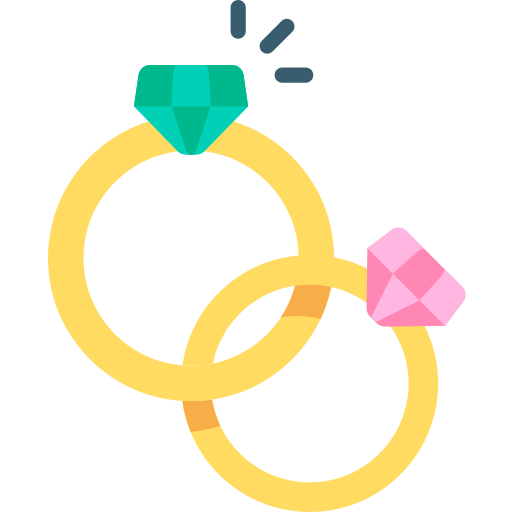
\includegraphics[width=.4\linewidth]{presentation/assets/marriage.png}
            \caption{MARRIAGE}
            \label{fig:sub4}
        \end{subfigure}%
        \begin{subfigure}{.165\textwidth}
            \centering
            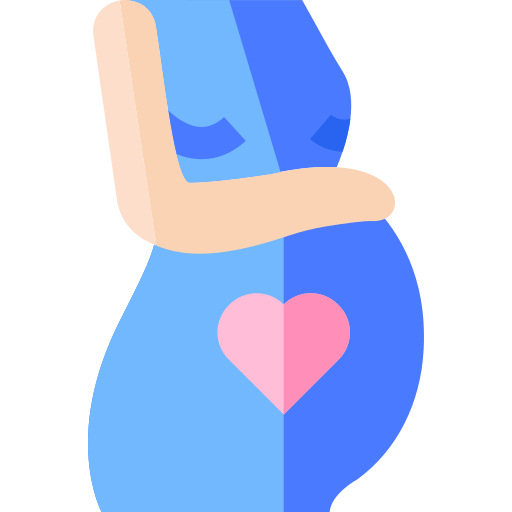
\includegraphics[width=.4\linewidth]{presentation/assets/pregnancy.png}
            \caption{PREGNANCY}
            \label{fig:sub5}
        \end{subfigure}%
        \begin{subfigure}{.165\textwidth}
            \centering
            
\includegraphics[width=.4\linewidth]{presentation/assets/religion.png}
            \caption{RELIGION}
            \label{fig:sub6}
        \end{subfigure}%
    \end{figure}
\end{frame}


\begin{frame}{Legal Perspective: ML and the current legal framework \cite{Barocas.2016}}
    \underline{\textbf{Issues inside the data mining process:}}\\
    \begin{itemize}
        \item \textbf{Target variable} must reflect judgments about what really is the problem (\textbf{inherit bias})
        \item \textbf{Compromise} between \textbf{forbidding} employers from using past discrimination and \textbf{allowing} them to use historical data of good employees
        \item \textbf{Skewed data sets} $\Rightarrow$ type of bias, possibility to \textbf{collect more} data
        \item Not accessible data $\Rightarrow$ \textbf{oversampling} underrepresented communities
        \item \textbf{Feature selection} statistical discrimination $\Rightarrow$ \textbf{additional} or \textbf{more granular data} (else: minimizing error rates between groups)
        \item \textbf{Proxies} $\Rightarrow$ \textbf{threshold} correlation between attribute and class membership becomes alarming \& when its still relevant enough to be used
    \end{itemize}
\end{frame}

% Short outlook of the rest of the day: Mathematical perspectives/solutions for questions of fairness
\section{Mathematical Perspective: How to quantify Fairness?}
\begin{frame}{Mathematical Perspective: How to quantify Fairness? \cite{Berk.2018}}
    \textbf{Question:} How to quantify unfairness inherent to machine learning mathematically? \\~\\
    $\Rightarrow$ Use confusion matrix as basis for fairness considerations
    \begin{table}[h]
    \label{tab:confusion}
    \centering
    \begin{tabular}{ c|c|c|c } 
    \toprule
      & \thead{$\hat{Y}_f$ \\ Failure Predicted} & \thead{$\hat{Y}_s$ \\ Success Predicted} & \thead{Conditional Procedure \\ Accuracy} \\ 
    \hline
    \thead{$Y_f$ \\ Failure - A Positive} & \makecell{$t_p$ \\ True Positive} & \makecell{$f_n$ \\ False Negative} & \makecell{$\frac{t_p}{t_p + f_n}$ \\ True Positive Rate} \\ 
    \hline
    \thead{$Y_s$ \\ Success - A Negative} & \makecell{$f_p$ \\ False Positive} & \makecell{$t_n$ \\ True Negative} & \makecell{$\frac{t_n}{t_n + f_p}$ \\ True Negative Rate } \\ 
    \hline
    \thead{Conditional \\ Use Accuracy} & \makecell{$\frac{t_p}{t_p + f_p}$ \\ Failure Prediction Accuracy} & \makecell{$\frac{t_n}{t_n + f_n}$ \\ Success Prediction Accuracy} & \makecell{$\frac{t_p + t_n}{t_p + f_p + t_n + f_n}$ \\ Overall Accuracy} \\ 
    \bottomrule
    \end{tabular}
    \end{table}
    
    \textbf{Idea:} Enforce equality of accuracy across protected subgroups
\end{frame}

\begin{frame}{Mathematical Perspective: How to quantify Fairness? \cite{Berk.2018}}
    
    \begin{itemize}
        \item \textbf{Overall accuracy equality:} equal probability of correct classification 
        \item \textbf{Statistical parity:} equal probability of predicting failure/success 
        \item \textbf{Conditional procedure accuracy equality:} equal probability of correct 
        classification, given the actual outcome
        \item \textbf{Conditional use accuracy equality:} equal probability of an actual 
        outcome, given the prediction
        \item \textbf{Treatment equality:} equal ratio between false negatives and positives
        \item \textbf{Total fairness:} All previously notions of fairness are achieved 
        simultaneously
    \end{itemize}
\end{frame}

\begin{frame}{Mathematical Perspective: How to quantify Fairness? \cite{Berk.2018}}
    \textbf{Problem:} Tradeoffs between accuracy and fairness \dots 

\begin{block}{\textbf{Fairness and accuracy:}\cite{Berk.2018}}
    \enquote{[\dots] excluding S will reduce accuracy. Any procedure that even just discounts the role of S will lead to less accuracy.}
\end{block}

\dots as well as between different kind of fairness necessary 

\begin{block}{\textbf{Impossibility Theorem:}\cite{Chouldechova2017FairPW, 
DBLP:journals/corr/KleinbergMR16}}
    \enquote{When the base rates 2 differ by protected group and when there is not separation 3 , one cannot have both conditional use accuracy and equality in the false negative and false positive rates.}
\end{block}

\end{frame}


\begin{frame}{Mathematical Perspective: How to quantify Fairness? \cite{Berk.2018}}
    Different technical solutions for creating fair machine learning proposed:
    
    \begin{itemize}
        \item \textbf{Pre-Processing}: elimination of sources of unfairness in the data before formulating $h(L,S)$
        \item \textbf{In-Processing}: including the adjustments for fairness in the process 
        of constructing $h(L,S)$
        \item \textbf{Post-Processing}: $h(L,S)$ is applied first, and its results are adjusted
        afterwards to account for fairness
    \end{itemize}
\end{frame}

{
\setbeamercolor{background canvas}{bg=gray}
\begin{frame}{Mathematical Perspective: How to quantify Fairness? \cite{Berk.2018}}
\vspace{2cm}
\begin{block}{\huge Overall:}
\LARGE 
    There is \textbf{no singular mathematical definition of fairness} and different definitions can be mutually exclusive. \\ 
    Accounting for fairness will always have an \textbf{impact on the overall prediction accuracy}.
\end{block}
\end{frame}
}

%\begin{frame}{Mathematical Perspective: How to quantify Fairness? \cite{Berk.2018}}
%    \begin{table}[h]
%    \centering
%    \begin{tabular}{ c|c|c|c } 
%    \toprule
%      & \thead{$\hat{Y}_f$ \\ Failure Predicted} & \thead{$\hat{Y}_s$ \\ Success Predicted} & \thead{Conditional Procedure \\ Accuracy} \\ 
%    \hline
%    \thead{$Y_f$ \\ Failure - A Positive} & \makecell{$t_p$ \\ True Positive} & \makecell{$f_n$ \\ False Negative} & \makecell{$\frac{t_p}{t_p + f_n}$ \\ True Positive Rate} \\ 
%    \hline
%    \thead{$Y_s$ \\ Success - A Negative} & \makecell{$f_p$ \\ False Positive} & \makecell{$t_n$ \\ True Negative} & \makecell{$\frac{t_n}{t_n + f_p}$ \\ True Negative Rate } \\ 
%    \hline
%    \thead{Conditional \\ Use Accuracy} & \makecell{$\frac{t_p}{t_p + f_p}$ \\ Failure Prediction Accuracy} & \makecell{$\frac{t_n}{t_n + f_n}$ \\ Success Prediction Accuracy} & \makecell{$\frac{t_p + t_n}{t_p + f_p + t_n + f_n}$ \\ Overall Accuracy} \\ 
%    \bottomrule
%    \end{tabular}
%    \end{table}
%    
%    \begin{onlyenv}<1>
%        \textbf{Overall accuracy equality:} equal probability of correct classification 
%    \end{onlyenv}
%    \begin{onlyenv}<2>
%        \textbf{Statistical parity:} equal probability of predicting failure/success 
%    \end{onlyenv}
%    \begin{onlyenv}<3>
%        \textbf{Conditional procedure accuracy equality:} equal probability of correct 
%        classification, given the actual outcome
%    \end{onlyenv}
%    \begin{onlyenv}<4>
%        \textbf{Conditional use accuracy equality:} equal probability of an actual 
%        outcome, given the prediction
%    \end{onlyenv}
%    \begin{onlyenv}<5>
%        \textbf{Treatment equality:} equal ratio between false negatives and positives 
%    \end{onlyenv}
%    \begin{onlyenv}<6>
%        \textbf{Total fairness:} All previously notions of fairness are achieved 
%        simultaneously
%    \end{onlyenv}
%\end{frame}

\section{Conclusion}
\begin{frame}{References}
    \nocite{*}
    \bibliographystyle{humannat}
    \bibliography{library}  
\end{frame}

\section{Concrete Example: Fairness in hiring decisions}
\begin{frame}{Concrete Example: Fairness in hiring decisions \cite{barocas-hardt-narayanan}}
\begin{columns}
\begin{column}{0.5\textwidth}
   \begin{itemize}
       \item In reality: non-linear model
       \item Two demographic groups: \textbf{triangles} and \textbf{squares}
       \item No consideration about group assignment
       \item Still: Triangles are higher performing and are more positively classified
   \end{itemize}
\end{column}
\begin{column}{0.5\textwidth}  %%<--- here
    \begin{figure}
        \centering
        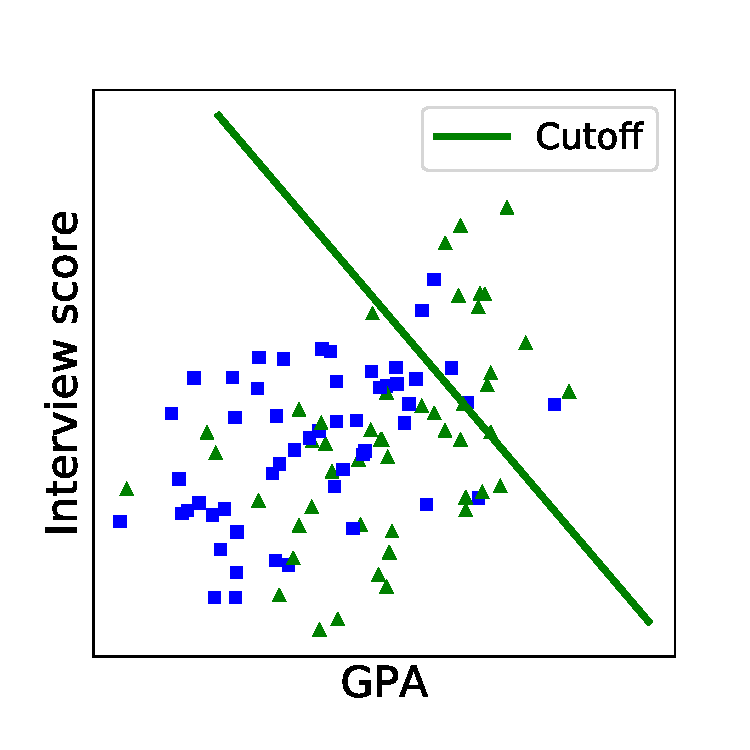
\includegraphics[width=.70\textwidth]{presentation/assets/toy_example.pdf}
        \caption{Hiring classifier that predicts job performance (not shown) based on GPA and interview score with a cutoff \cite{barocas-hardt-narayanan}}
        \label{fig:my_label}
    \end{figure}
\end{column}
\end{columns}
\end{frame}

\begin{frame}{Concrete Example: Fairness in hiring decisions \cite{barocas-hardt-narayanan}}
    \begin{columns}
\begin{column}{0.5\textwidth}
\underline{\textbf{Reasons for Disparities:}}\newline 

   \begin{itemize}
       \item Managers who score performance might have bias against one group
       \item Workplace biased, preventing group from reaching their full potential
       \item Disparities in educational institutions attended
   \end{itemize}
\end{column}
\begin{column}{0.5\textwidth}  %%<--- here
    \begin{figure}
        \centering
        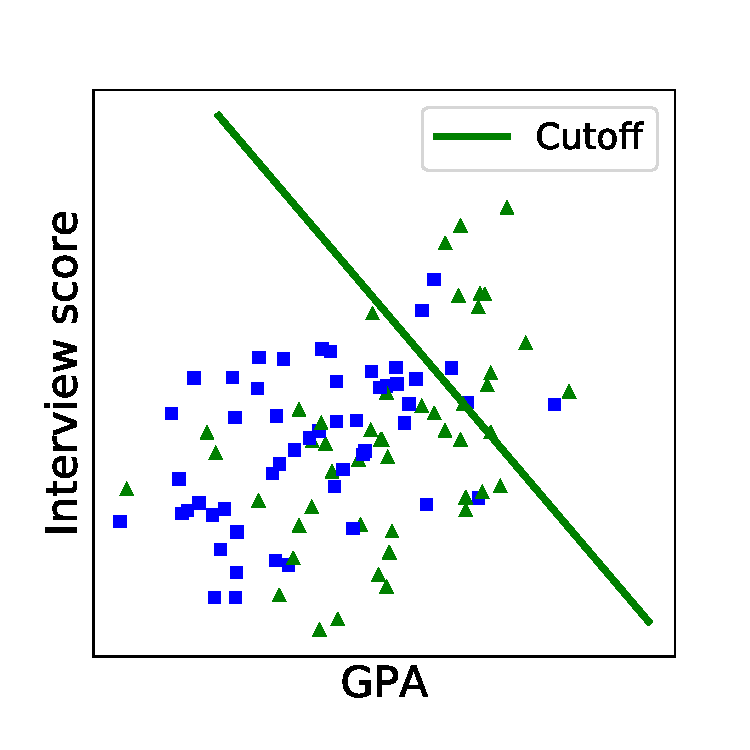
\includegraphics[width=.70\textwidth]{presentation/assets/toy_example.pdf}
        \caption{Hiring classifier that predicts job performance (not shown) based on GPA and interview score with a cutoff \cite{barocas-hardt-narayanan}}
        \label{fig:my_label}
    \end{figure}
\end{column}
\end{columns}
\end{frame}

\begin{frame}{Concrete Example: Fairness in hiring decisions \cite{barocas-hardt-narayanan}}
    \begin{columns}
\begin{column}{0.5\textwidth}
\underline{\textbf{Solving unjustified Disparities:}}\newline 

   \begin{itemize}
       \item GPA proxy for demographic group (dropping it would result in a loss of accuracy)
       \item Using different cutoffs for hiring so both groups have same probability of being hired (which cutoffs?)
       \item \underline{Generally:} Many algorithmic possibilities especially \textbf{similarity function between pairs of individuals}
   \end{itemize}
\end{column}
\begin{column}{0.5\textwidth}  %%<--- here
    \begin{figure}
        \centering
        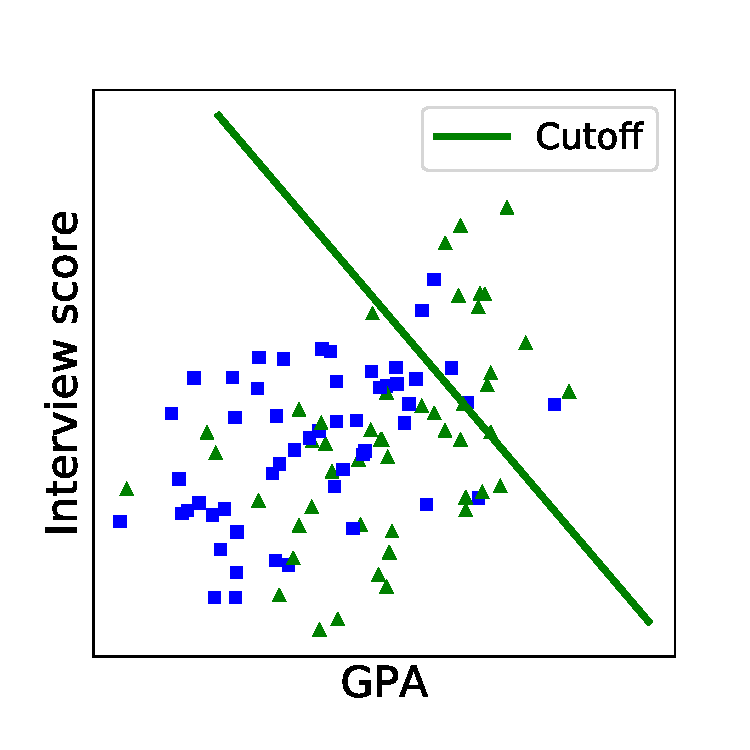
\includegraphics[width=.70\textwidth]{presentation/assets/toy_example.pdf}
        \caption{Hiring classifier that predicts job performance (not shown) based on GPA and interview score with a cutoff \cite{barocas-hardt-narayanan}}
        \label{fig:my_label}
    \end{figure}
\end{column}
\end{columns}
\end{frame}


\end{document}